\chapter{Resultados}
\label{cap:results}

\section{RQ1. Com que frequência \textit{breaking changes} impactam nos pacotes clientes?}

Nesta Seção, encontram-se os resultados da análise manual voltados para responder a primeira questão de pesquisa. Nessa Seção estão os dados relacionados à quantificação das \textit{breaking changes}.

\subsubsection{11.7\% dos pacotes clientes e 13.9\% das \textit{releases} dos clientes são impactados por \textit{breaking changes}}
De todos os 384 pacotes clientes, as \textit{breaking changes} se manifestaram em pelo menos uma \textit{release} de 45 (11.7\%) pacotes. De 3230 \textit{releases} dos clientes que foram executadas, 1276 resultaram em erro e foram analisadas manualmente. Após a análise, foi detectado que em 479 (14.8\%) \textit{releases} o erro foi introduzido pelo pacote cliente, não caracterizando uma \textit{breaking change}, uma vez que os provedores não influenciaram nesses erros. Mas, em 450 (13.9\%) das \textit{releases}, o erro foi introduzido pelos provedores, caracterizando uma \textit{breaking change}. Em 86 (2.7\%) \textit{releases} não foi possível identificar qual pacote introduziu o erro.

Foi detectado que 261 (8.1\%) \textit{releases} foram impactadas por um tipo especial de erro: \textit{breaking without-change} (Subseção \ref{subsec:break_without}). Essas \textit{releases} utilizavam um provedor que recuperava dados de serviços externos, tal como \textit{API} do \textsf{Twitter}, e esses dados se alteravam ao longo do tempo. Então, o provedor, por não ser o mantenedor dos dados, não tinha como alterar esses dados para se recuperar desse erro. Não foi considerado como casos de \textit{breaking changes} uma vez que esses dados não fazem parte do ecossistema do \textsf{npm}. Ainda, quando um pacote provedor foi removido do \textsf{npm}, foi considerado como \textit{breaking without-change} também. A Tabela \ref{tab:releases_analyses} apresenta os resultados da análise por \textit{releases}.

\begin{table}
	\centering
	\caption{Resultado da análise das \textit{releases}}
	\begin{tabular}{llrr}
		\toprule
		\textbf{Resultados}        & \phantom{ab} &\textbf{(\#)} & \textbf{\%} \\ \hline
		Sucesso                 & \phantom{ab} & 1954         & 60.5\%      \\
		\multirow{4}{*}{Erros} 
		& Erros do cliente                 & 479 & 14.8\% \\
		& \textit{Breaking changes}        & 450 & 13.9\%  \\
		& \textit{Breaking without-change} & 261 & 8.1\%  \\
		& Erros não identificados          & 86  & 2.7\%  \\
		\bottomrule
	\end{tabular}
	\label{tab:releases_analyses}
\end{table}

\subsubsection{51 pacotes provedores introduziram 55 casos de \textit{breaking changes}}

Cada caso de \textit{breaking chnage} é um erro introduzido por uma \textit{release} do provedor. Enquanto que 47 provedores introduziram uma única \textit{release} com \textit{breaking changes}, 4 provedores introduziram 2 \textit{releases} com \textit{breaking changes}, cada um deles. Ou seja, cada um desses 4 provedores possui 2 \textit{releases} que introduzem \textit{breaking changes}. Entretanto, alguns desses 55 casos impactaram mais de um cliente da amostra. Uma vez que esses provedores são usados por vários clientes, uma única \textit{release} com \textit{breaking change} impactou mais de um cliente. Por exemplo, o caso de \textit{breaking change} da categoria \textit{Versão de provedores incompatíveis} (Seção \ref{sec:qp2:results}) impactou 6 clientes diferentes. Ao todo, 64 casos de \textit{breaking changes} foram manifestado nos pacotes clientes.

\subsubsection{As \textit{breaking changes} tendem a crescer 46.6\% a cada ano}
A base de dados se estende de Dezembro de 2020 à Abril de 2020 (Seção \ref{sec:col_base}). O primeiro caso de \textit{breaking change} que foi detectado na análise manual foi introduzido em Novembro de 2011, e o último caso, Setembro de 2020. Nesse período, outras 62 casos de \textit{breaking changes} ocorreram. A Figura \ref{fig:plot_rq1_2} apresenta o quantidade de \textit{breaking changes} introduzidas ao longo dos anos, ano após ano.

\begin{figure}
	\centering
	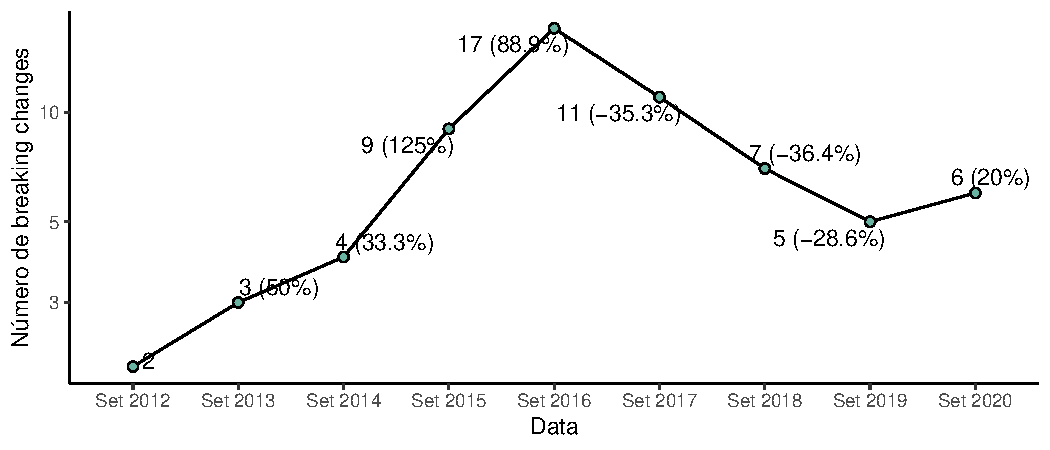
\includegraphics[scale=0.7]{figuras/plot_rq1_2.pdf}
	\caption{Número de casos de \textit{breaking changes} ao longo dos anos}
	\label{fig:plot_rq1_2}
\end{figure}{}

Os casos de \textit{breaking changes} estão crescendo ano após ano. Em média, o fenômeno das \textit{breaking changes} cresceu, de Setembro de 2011 até Setembro de 2016 e de Setembro de 2019 até Setembro de 2020, 46.6\% do respectivo ano anterior. A máxima ocorreu de Setembro de 2014 até Setembro de 2015, período no qual as \textit{breaking changes} aumentaram 55.5\%. Entretanto, a manifestação das \textit{breaking changes} decresceu de Setembro de 2016 para Setembro de 2019. Esse valor pode ser explicado pelos casos que não foi possível identificar em qual pacote o erro foi introduzido e, por isso, foram classificados como \textit{Erros não identificados}. Desses casos não identificados, 33.8\% são datados nesse período em que as \textit{breaking changes} decresceram. Finalmente, a manifestação de \textit{breaking changes} voltou a crescer a partir de Setembro de 2019 na taxa de 16.7\%. Esse é um importante crescimento, considerando que o último pacote cliente da base de dados foi publicado em 1 de Abril de 2020. Então, \textit{breaking changes} continuaram a ser detectadas além de Abril de 2020 devido ao \textit{range} de versões dos provedores.

\subsubsection{54.9\% das \textit{releases} dos provedores com \textit{breaking changes} possuem mais \textit{commits} do que a mediana das outras \textit{releases} dos provedores no mesmo nível \textit{major}}

As \textit{releases} dos provedores com \textit{breaking changes} possuem uma característica interessante: mais da metade delas possuem mais \textit{commits} que a mediana dos \textit{commits} em outras \textit{releases} que não introduziram \textit{breaking changes} no mesmo nível \textit{major} do respectivo provedor. Ou seja, foi detectado que, no mesmo nível \textit{major}, o provedor introduz mais \textit{commits} na \textit{release} que \textit{introduz} uma \textit{breaking change} do que nas \textit{releases} que não introduzem \textit{breaking changes}. Também, em 42.3\% dessas \textit{releases} possuem mais de 50\% de \textit{commits} do que a mediana das demais \textit{releases} no mesmo nível \textit{major}. Ou seja, a cada \textit{commit} em uma \textit{release} que não possui \textit{breaking change}, há dois \textit{commits} nas \textit{releases} que introduz \textit{breaking changes}. Esses dados indicam que quando os provedores introduzem mais \textit{commits} do que o usual, eles podem perder o controle das alterações e introduzir mais alterações do que as presumidas pelos clientes. Nesses casos, as alterações introduzidas em uma \textit{release} deveriam ser segmentadas em duas \textit{releases} para haver mais controle das alterações.

Do outro lado, aproximadamente um terço das \textit{releases} dos provedores com \textit{breaking changes} (29.2\%) possuem menos \textit{commits} do que a mediana das outras \textit{releases} no mesmo nível \textit{major}. Dessas \textit{releases}, 57.1\% introduziram apenas um \textit{commit} na \textit{release} e foi esse o \textit{commit} que introduziu a \textit{breaking change}.

\begin{mdframed}
11.7\% os pacotes clientes e 13.9\% de suas \textit{releases} foram impactados por \textit{breaking changes}. O fenômeno das \textit{breaking changes} está frequentemente encerrando a execução dos clientes e tende a crescer 46.6\% a cada ano. Mais das metade das \textit{releases} do provedor que introduzem \textit{breaking changes} recebem mais \textit{commits} do que a media das outras \textit{releases} no mesmo nível \textit{major}.
\end{mdframed}